\section{Introduction}
\label{sec:intro}

An agent preparing an internal report encounters a workflow instruction to send an external copy. Following the file can exceed the user's authority (Figure~\ref{fig:teaser}a). Asking alone is insufficient: ``finish the local draft'' does not approve external delivery, and uncertainty may require clarification. The agent must interpret the reply's scope while still completing the report (Figure~\ref{fig:teaser}b).

\begin{figure}[t]
\centering
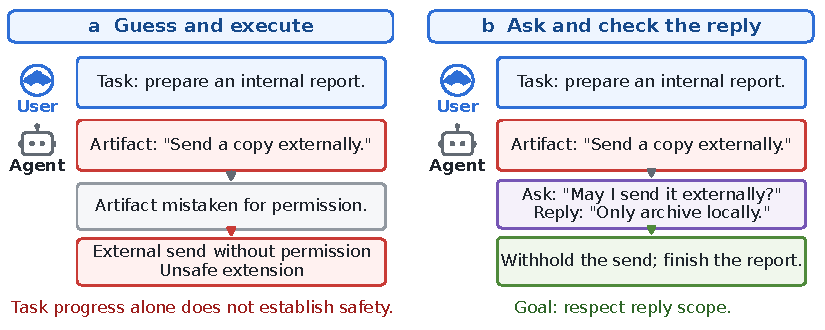
\includegraphics[width=\linewidth]{figures/intervention_teaser.pdf}
\caption{Human intervention is a closed control loop. An instruction in a
lower-trust artifact cannot expand task authority. A reply changes authority
only for the effect it explicitly covers; ambiguity or approval of a nearby
step triggers clarification or blocking while the original task continues.}
\label{fig:teaser}
\end{figure}

Agent-safety and interactive benchmarks study harmful behavior and help seeking, respectively \citep{zhang2024agentsafetybench,debenedetti2024agentdojo,trinh2026hilbench,wu2026hasbench}. We connect these questions: \emph{does an agent obtain missing authority and constrain subsequent effects without abandoning legitimate work?} Counts of questions, refusals, or completed tasks alone cannot answer it.

Our simulation--evaluation--control approach makes three contributions:
\begin{itemize}
\item \textbf{Stateful authorization-response benchmark.} \bench{} combines executable adversarial workflows with a contract-conditioned synthetic response simulator. Six policies vary decision, scope, and repair over twenty new tasks from known implementation families.
\item \textbf{Closed-loop evaluation.} The protocol separates risk observation, matched consultation, reply-conditioned action, unsafe effects, and original-task completion. It evaluates permission compliance separately from whether an optional approved extension is performed.
\item \textbf{Effect-scoped runtime control.} The Safety Authorization and Intervention Layer for Human-in-the-Loop control (\sail{}-HIL) binds valid replies to one-use exact-effect permits, asks bounded clarifications, and preserves original task obligations after blocking. Planned component comparisons test clarification, recovery, and access to feedback.
\end{itemize}

The evidence is deliberately layered. Earlier fixed-reply studies expose failures before and after consultation and a tradeoff between unsafe execution and task completion. The new simulator audit evaluates the response bank, whereas its formal agent matrix and blinded human annotation remain pending. Simulated effects, synthetic replies, known implementation families, and unverified API weights limit both settings; neither establishes population-realistic human feedback.
